% !TEX program = xelatex
\documentclass{ctexart}
\usepackage{listings}
\usepackage{mathtools}
\usepackage{ctex}
\usepackage{xcolor}
\lstset{
    basicstyle          =   \sffamily,          % 基本代码风格
    keywordstyle        =   \bfseries,          % 关键字风格
    commentstyle        =   \rmfamily\itshape,  % 注释的风格,斜体
    stringstyle         =   \ttfamily,          % 字符串风格
    flexiblecolumns,                            % 别问为什么,加上这个
    numbers             =   left,               % 行号的位置在左边
    showspaces          =   false,              % 是否显示空格,显示了有点乱,所以不现实了
    numberstyle         =   \zihao{-5}\ttfamily, % 行号的样式,小五号,tt等宽字体
    showstringspaces    =   false,
    captionpos          =   t,      % 这段代码的名字所呈现的位置,t指的是top上面
    frame               =   lrtb,   % 显示边框
}

\usepackage{amsmath,amsthm,amssymb}
\usepackage{autobreak}
\usepackage{hyperref}
\usepackage{booktabs}
\usepackage{geometry}
\usepackage{appendix}
\usepackage{multicol}
\usepackage{subfig,graphicx}
\usepackage{listings}
\newtheorem{attention}{注意}
\newtheorem{definition}{定义}[section]
\newtheorem{theorem}{定理}[section]
\newtheorem{inference}{推论}[section]
\newtheorem{xingzhi}{性质}
\newcommand{\upcite}[1]{\textsuperscript{\textsuperscript{\cite{#1}}}}
\newcommand*{\dif}{\mathop{}\!\mathrm{d}}
\def\degree{${}^{\circ}$}
%%%%%%%%%%%%%%%%%%%%%%%
%  设置水印
%%%%%%%%%%%%%%%%%%%%%%%
%\usepackage{draftwatermark}         % 所有页加水印
%\usepackage[firstpage]{draftwatermark} % 只有第一页加水印
% \SetWatermarkText{Water-Mark}           % 设置水印内容
% \SetWatermarkText{\includegraphics{fig/ZJDX-WaterMark.eps}}         % 设置水印logo
% \SetWatermarkLightness{0.9}             % 设置水印透明度 0-1
% \SetWatermarkScale{1}                   % 设置水印大小 0-1

\author{张阳}
\date{\today}
\title{三次样条插值}
\numberwithin{equation}{section}
\geometry{left=2.0cm, right=2.0cm, top=2.5cm, bottom=2.5cm}

%\punctstyle{quanjiao}全角式,所有标点全角。例如,“标点挤压”。又如《标点符号用法》。 
%\punctstyle{banjiao}半角式,所有标点半角。例如,“标点挤压”。又如《标点符号用法》。 
%\punctstyle{kaiming}开明式,部分的标点半角。例如,“标点挤压”。又如《标点符号用法》。 
%\punctstyle{hangmobianjiao}行末半角式,仅行末挤压。例如,“标点挤压”。又如《标点符号用法》。 
%\punctstyle{plain}无格式,只有禁则,无挤压。例如,“标点挤压”。又如《标点符号用法》。

\begin{document}
\maketitle
\tableofcontents
\newpage
\section{问题的引出}
当多项式次数较大时 ($n\geqslant8$),使用多项式拟合函数 $f(x)$ 就会产生龙格现象。
\begin{figure}[htp]
    \centering
    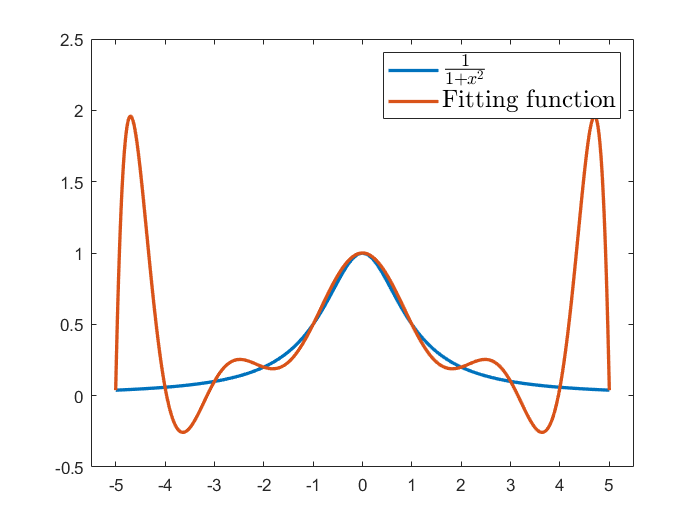
\includegraphics[width=0.7\linewidth]{fig/龙格现象}
    \caption{图为 $y=\frac{1}{1+x^2}$ 与 $10$ 阶多项式拟合函数}
    \label{fig:1}
\end{figure}

为了避免高次多项式函数带来的龙格现象,又保留多项式函数的良好性质,我们采用了分段低次拟合的方法。

有定理已经证明,分段线性插值函数可在插值区间上一致收敛到原函数。

但是,分段线性插值函数在插值点处大多数情况下不可导,这就导致了拟合的函数不够光滑。因此,我们引入了三次样条插值。
\begin{figure}[htp]
    \centering
    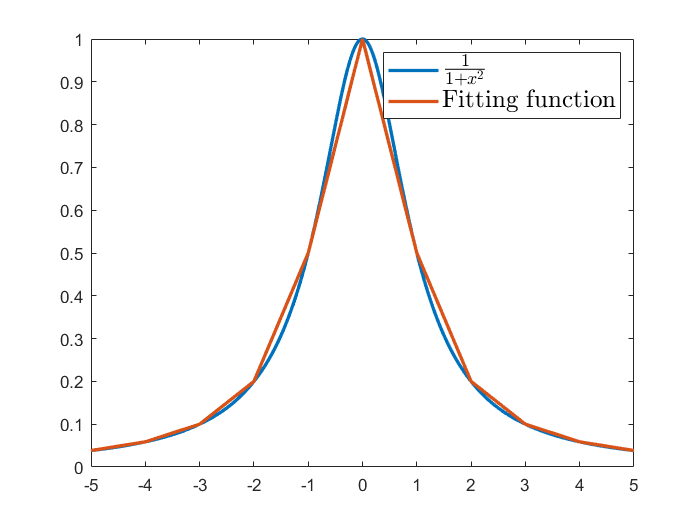
\includegraphics[width=0.7\linewidth]{fig/分段线性插值}
    \caption{图为 $y=\frac{1}{1+x^2}$ 与 线性插值拟合函数}
    \label{fig:2}
\end{figure}
\section{三次样条插值的性质}



\begin{definition}
    若函数 $S(x)\in C^2[a,b]$ 且在每个小区间 $[x_j,x_{j+1}]$ 上是三次多项式,其中 $a=x_0<x_1<\cdots<x_n=b$ 是给定节点,则称 $S(X)$ 是节点 $x_0,x_1,\cdots,x_n$ 上的三次样条函数,若在节点 $x_j$ 上给定函数值 $y_j = f(x_j)(j=0,1,\cdots,n)$,并成立

    \begin{equation}
        S(x_j)=y_j,\quad j=0,1,\cdots,n,
    \end{equation}
    则称 $S(x)$ 为三次样条插值函数。记 $S_i(x)=S(x)|_{x\in [x_i,x_{i+1}]}$。
\end{definition}

三次样条插值的特点是:在避免了龙格现象的同时,又使得插值函数具有良好的光滑性。

由定义知,$S(X)$ 在 $[a,b]$ 上的二阶导数连续(显然一阶导数和原函数也连续),于是应当满足
\begin{equation}
\begin{aligned}
     &S_{a} = y_0\\
    &S_{b} = y_n\\
    &S_{i-1}(x_i) = S_{i}(x_i) = y_i,\quad i = 1,2,\cdots,n-1\\
    &S'_{i-1}(x_i) = S'_{i}(x_i),\quad i = 1,2,\cdots,n-1\\
     &S''_{i-1}(x_i) = S''_{i}(x_i),\quad i = 1,2,\cdots,n-1
\end{aligned}
\label{eq:1}
\end{equation}

共有 $n$ 个三次函数,所以有 $4n$ 个未知参数求解,而 \eqref{eq:1} 中共有 $4n-2$ 个等式。

为了求出确定的样条插值函数,还需给定 $2$ 个条件。常用的条件有:

\begin{enumerate}
    \item $S''_0(x_0)=S''_{n-1}(x_n)=0$ 这样构造出来的样条称为自然样条
    \item $S''_0(x_0)=u,S''_{n-1}(x_n)=v$ 这样构造出来的样条称为曲率调整三次样条
    \item $S'_0(x_0)=u,S'_{n-1}(x_n)=v$ 这样构造出来的样条称为钳制三次样条
    \item $S_0,S_{n-1}$ 均为至多二阶,这样构造出来的样条称为抛物线端点的三次样条
\end{enumerate}
下面详细介绍钳制三次样条的求解方法。
\section{钳制三次样条的求解方法}
设
\begin{equation}
    S'_{i-1}(x_i) = S'_{i}(x_i)=m_{i-1},\quad i = 2,3,\cdots,n-1
\end{equation}

为形式上的统一,令 $u = m_0,v = m_n$

于是有

\begin{table}[htp]
    \begin{center}
        \begin{tabular}{cccccc}
        \toprule
        & $x_0$ & $x_1$ & $x_2$ & $\cdots$ & $x_n$ \\ 
        \midrule
        $f(x)$  & $y_0$ & $y_1$ & $y_2$ & $\cdots$ & $y_n$ \\ 
        $f'(x)$ & $m_0$ & $m_1$ & $m_2$ & $\cdots$ & $m_n$ \\ 
        \bottomrule
        \end{tabular}
    \end{center}
\end{table}

则 

\begin{equation}
\begin{aligned}
    s_i(x) 
    & = \frac{\left(x-x_{i+1}\right)^{2}\left[h_{i}+2\left(x-x_{i}\right)\right]}{h_{i}^{3}} y_{i}\\
    & +\frac{\left(x-x_{i}\right)^{2}\left[h_{i}+2\left(x-x_{i+1}\right)\right]}{h_{i}^{3}} y_{i+1} \\
    & + \frac{\left(x-x_{i+1}\right)^{2}\left(x-x_{i}\right)}{h_{i}^{2}} m_{i}\\
    & +\frac{\left(x-x_{i}\right)^{2}\left(x-x_{i+1}\right)}{h_{i}^{2}} m_{i+1}\qquad i = ,0,1\cdots,n-1
    \end{aligned}
\label{eq:8}\end{equation}
其中 $h_i = x_{i+1}-x_i$

\begin{attention}
    这里求 $S_i(x)$ 用到了埃尔米特插值的基函数的方法。
\end{attention}

为了解出 $m_i$,就要用到二阶导数连续的性质。
\begin{equation}
\begin{aligned}
    S_i''(x) &=\frac{6 x-2 x_{i}-4 x_{i+1}}{h_{i}^{2}} m_{i} \\
    &+\frac{6 x-4 x_{i}-2 x_{i+1}}{h_{i}^{2}} m_{i+1} \\
    &+\frac{6\left(x_{i}+x_{i+1}-2 x\right)}{h_{i}^{3}}\left(y_{i+1}-y_{i}\right)\quad,i = 0,1,\cdots,n-1
    \end{aligned}
\end{equation}
从而

\begin{equation}
    \begin{aligned}
    &S''_i(x_i) = -\frac{4}{h_i}m_i-\frac{2}{h_i}m_{i+1}+\frac{6}{h^2_i}(y_{i+1}-y_i)\\
    &S''_i(x_{i+1}) = \frac{2}{h_i}m_i+\frac{4}{h_i}m_{i+1}-\frac{6}{h^2_i}(y_{i+1}-y_i)\\
    \end{aligned}
    \quad,i = 0,1,\cdots,n-1
\end{equation}

由二阶导数连续的条件,有:

\begin{equation*}
    -\frac{4}{h_i}m_i-\frac{2}{h_i}m_{i+1}+\frac{6}{h_i}(y_{i+1}-y_i)
    = \frac{2}{h_{i-1}}m_{i-1}+\frac{4}{h_{i-1}}m_{i}-\frac{6}{h_{i-1}}(y_{i}-y_{i-1}) \quad,i = 1,2,\cdots,n-1
   \end{equation*}

整理得到:

\begin{equation}
    \frac{1}{h_{i-1}} m_{i-1}+2\left(\frac{1}{h_{i-1}}+\frac{1}{h_{i}}\right) m_{i}+\frac{1}{h_{i}} m_{i+1} =3\left(\frac{y_{i+1}-y_{i}}{h_{i}^{2}}+\frac{y_{i}-y_{i-1}}{h_{i-1}^{2}}\right) \quad(i=1,2,\cdots, n-1)
    \label{eq:3}
\end{equation}

令 
\begin{equation}
    \lambda_i = \dfrac{\frac{1}{h_{i-1}}}{\frac{1}{h_{i-1}}+\frac{1}{h_i}} \quad
    \mu_i = \dfrac{\frac{1}{h_i}}{\frac{1}{h_{i-1}}+\frac{1}{h_i}} \quad
    g_i = 3\dfrac{\frac{y_{i+1}-y_{i}}{h_{i}^{2}}+\frac{y_{i}-y_{i-1}}{h_{i-1}^{2}}}{\frac{1}{h_{i-1}}+\frac{1}{h_i}}
    \label{eq:7}
\end{equation}

于是 \eqref{eq:3} 可进一步化简为

\begin{equation}
    \lambda_i m_{i-1}+2m_i+\mu_i m_{i+1} = g_i\quad(i=1,2,\cdots, n-1)
\end{equation}

写成矩阵形式为

\begin{equation}
    \begin{bmatrix}
    2 & \mu_{1} & 0 & \cdots & 0 & 0 & 0 \\
    \lambda_{2} & 2 & \mu_{2} & \cdots & 0 & 0 & 0 \\
    0 & \lambda_{3} & 2 & \cdots & 0 & 0 & 0 \\
    \vdots & \vdots & \vdots & \vdots & \vdots & \vdots & \vdots \\
    0 & 0 & 0 & \cdots & 2 &  \mu_{n-1} & 0 \\
    0 & 0 & 0 & \cdots & \lambda_{n-2} & 2 & \mu_{n-2} \\
    0 & 0 & 0 & \cdots & 0 & \lambda_{n-1} & 2
\end{bmatrix}\begin{bmatrix}
    m_{1} \\
    m_{2} \\
    m_{3} \\
    \vdots \\
    m_{n-3} \\
    m_{n-2} \\
    m_{n-1}
\end{bmatrix}  = 
    \begin{bmatrix}
    g_{1}-\lambda_{1} f_{0}^{\prime} \\
    g_{2} \\
    g_{3} \\
    \vdots \\
    g_{n-3} \\
    g_{n-2} \\
    g_{n-1}-\mu_{n-1} f_{n}^{\prime}
\end{bmatrix}
\label{eq:4}
\end{equation}

求解线性方程组 \refeq{eq:4} 即可解出 $m_1,m_2,\cdots,m_{n-1}$ 从而算出 $s_i(x)$

\begin{attention}
    此方程为严格对角占优矩阵,可用追赶法求解。
\end{attention}
\section{示例演示}
\begin{itemize}
    \item 根据下列数据点,求出三次样条插值多项式
    \item 利用三次样条插值多项式计算当 $x = 3.5$ 时,$y$ 的拟合值
\end{itemize}
\begin{table}[htp]
    \begin{center}
    \begin{tabular}{ccccccccc}
    \toprule
    $x$     & 1      & 2    & 3    & 4     & 5     & 6     & 7     & 8       \\
    \midrule
    $f(x)$  & 0.84   & 0.91 & 0.14 & -0.76 & -0.96 & -0.28 & -0.66 & 0.99    \\
    $f'(x)$ & $0.5403$ &      &      &       &       &       &       & -0.1455  \\
    \bottomrule
    \end{tabular}
    \end{center}
    \end{table}
    利用公式 \eqref{eq:7},\eqref{eq:4},可以得到关于 $m_i$ 的线性方程组。

    \begin{equation}
        \begin{bmatrix}
            2 & 0.5 & 0 & 0 & 0 & 0 \\
            0.5 & 2 & 0.5 & 0 & 0 & 0 \\
            0 & 0.5 & 2 & 0.5 & 0 & 0 \\
            0 & 0 & 0.5 & 2 & 0.5 & 0 \\
            0 & 0 & 0 & 0.5 & 2 & 0.5 \\
            0 & 0 & 0 & 0 & 0.5 & 2
            \end{bmatrix}
            \begin{bmatrix}
                    m_1\\
                    m_2\\
                    m_3\\
                    m_4\\
                    m_5\\
                    m_6\\
                \end{bmatrix}=
                \begin{bmatrix}
                    -1.3201 \\
                    -2.5050 \\
                    -1.6500 \\
                    0.7200 \\
                    2.4300 \\
                    1.9778
                    \end{bmatrix}
    \end{equation}
    解得:
    \[m = [0.5403,-0.4133 ,-0.9869,-0.6490,0.2831,0.9568,0.7497,-0.1455]^T\]
    带入 \eqref{eq:8},即可得到:

    \begin{small} 
    \begin{equation}   
        S(x) = \left\{
        \begin{aligned}
            &0.84(x-2)^{2}(2 x-1)-0.91(x-1)^{2}(2 x-5)+0.54(x-1)(x-2)^{2}-0.41(x-1)^{2}(x-2) \quad x\in(1,2)\\
            &0.91(x-3)^{2}(2 x-3)-0.99(x-2)^{2}(x-3)-0.14(x-2)^{2}(2 x-7)-0.41(x-2)(x-3)^{2} \quad x\in(2,3)\\
            &0.14(x-4)^{2}(2 x-5)-0.99(x-4)^{2}(x-3)-0.65(x-4)(x-3)^{2}+0.76(x-3)^{2}(2 x-9) \quad x\in(3,4)\\
            &0.96(x-4)^{2}(2 x-11)-0.76(x-5)^{2}(2 x-7)-0.65(x-4)(x-5)^{2}+0.28(x-4)^{2}(x-5) \quad x\in(4,5)\\
            &0.28(x-5)(x-6)^{2}+0.96(x-5)^{2}(x-6)-0.96(x-6)^{2}(2 x-9)+0.28(x-5)^{2}(2 x-13) \quad x\in(5,6)\\
            &0.96(x-6)(x-7)^{2}+0.75(x-6)^{2}(x-7)-0.28(x-7)^{2}(2 x-11)-0.66(x-6)^{2}(2 x-15) \quad x\in(6,7)\\
            &0.75(x-8)^{2}(x-7)-0.15(x-8)(x-7)^{2}+0.66(x-8)^{2}(2 x-13)-0.99(x-7)^{2}(2 x-17)\quad x\in(7,8)
            \end{aligned}\right.
    \end{equation}
\end{small}
于是 $S(3.5)=-0.3522$
\begin{figure}[htp]
    \centering
    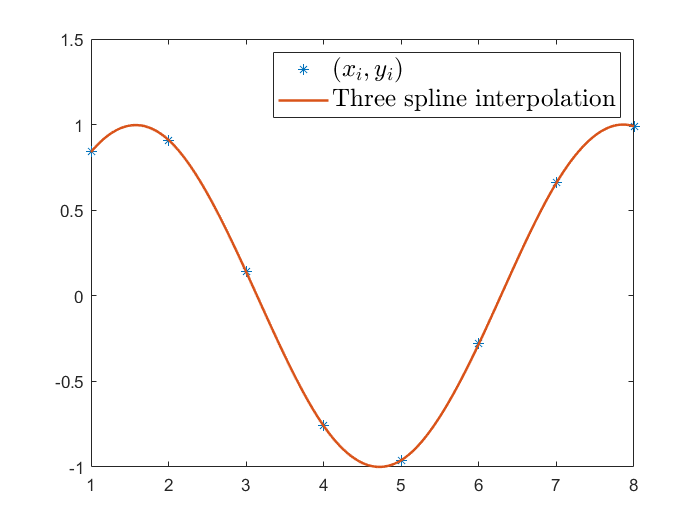
\includegraphics[width=0.7\linewidth]{fig/三次样条插值}
    \caption{插值点与插值函数}
\end{figure}
\newpage
\section{代码附录}
\begin{appendices}
    \lstinputlisting[caption={\bf main.m},]{code/main.m}
    \lstinputlisting[caption={\bf get\_m.m},]{code/get_m.m}
    \lstinputlisting[caption={\bf my\_elmit.m},]{code/my_elmit.m}
\end{appendices}
\end{document}